%parent:def:heegaardSplitting
%author:JeffHicks
%name:"Heegaard splitting"
%type:"example"
%indepth:art:heegaardDiagram
%label:"exm:heegaardSplitting"


    Consider the 3-sphere
    \[M=S^3=\left\{(x_0, x_1, x_2, x_3)\st x_i\in \RR, \sum_{i=1}^3 x_i^2=1.\right\}\]
    Consider the decomposition of this into two halves along the $z_0$ coordinate:
    \begin{align*}
        U_1=\{(x_0, x_1, x_2, x_3)\in S^3 \st x_0\leq 0\}&& U_2=\{(x_0, x_1, x_2, x_3)\in S^3 \st x_0\geq 0\}
    \end{align*}
    Then both $U_1, U_2$ are diffeomorphic to the 3-ball, and are glued together by their common boundary $S^2=\Sigma_0$. See \cref{fig:heegaardSplitting}.
    %parent:def:heegaardSplitting
%author:JeffHicks
%name:"Heegaard splitting for $S^3$"
%type:"figure"
%indepth:art:heegaardDiagram
%label:"fig:heegaardSplitting"
%parent:"exm:heegaardSplitting"
%caption:"After identifying $S^3\setminus \{(1, 0, 0, 0)\}$ with $\RR^3$ via stereographic projection, the Heegaard splitting of $S^3$ is given by taking the unit sphere, which decomposes the sphere into two $3$-balls. We also draw the meridinal line $(\cos(\theta), \sin(\theta), 0, 0)$."



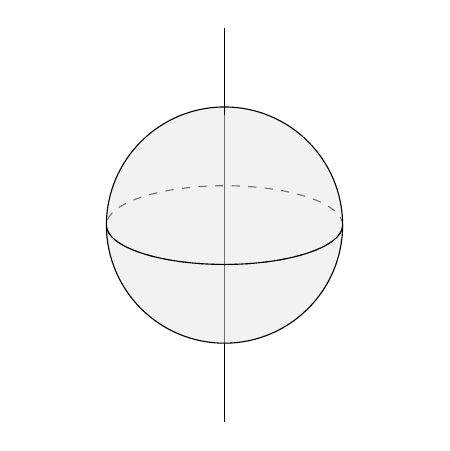
\begin{tikzpicture}
    \draw (-0.5,2) -- (-0.5,-3);
    \draw[dashed]  (-0.5,-0.5) ellipse (1.5 and 0.5);
    \draw[fill=gray!20, fill opacity=.5]  (-0.5,-0.5) ellipse (1.5 and 1.5);
    
    \draw (-0.5,2) -- (-0.5,0.9);
    
    \clip  (2,-0.5) rectangle (-3,-1.5);
    \draw  (-0.5,-0.5) ellipse (1.5 and 0.5);
    \end{tikzpicture}
    \label{exm:heegaardSplitting}
